\graphicspath{ {imgs/} }
\documentclass[main.tex]{subfiles}
\begin{document}
\chapter{Current Approaches}\label{chap:approaches}
This chapter illustrates the current state of the art in the field of automated nodule detection. Roughly the field can be divided among the used methods in the \emph{classical} approaches and the deep learning approaches. It also describes how this thesis is situated in the field and what is done differently compared to previous papers.

\section{Classical Approaches}
Nodule detection is a complex and potentially life-saving task, so it makes sense that there is a scientific community dedicated to finding algorithmic approaches to aid the radiologists. In this section some of the published papers in this domain and the techniques they use will be explained. In principal algorithms applied to the lung CT images can be subdivided in several stages (as can be for example seen in~\ref{fig:pipeline}). Similar to other computer vision algorithms those can be roughly clustered in the following: Segmentation, Candidate Selection, Classification.


\begin{figure}[ht]
\centering
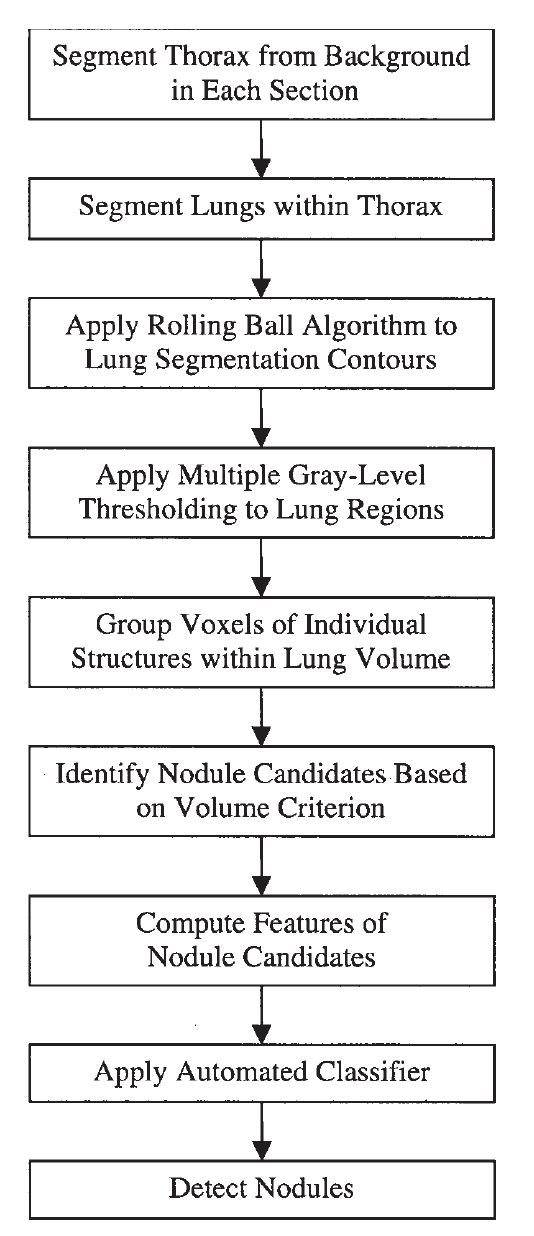
\includegraphics[scale=0.5]{armato_pipeline.png}
\caption{This image is taken from Armato's paper ``Computerized Detection
of Pulmonary Nodules on CT Scans''~\cite{armato1999computerized} and describes on one specific example how a traditional approach towards nodule detection is modeled.}
\label{fig:pipeline}
\end{figure}


\subsection{Segmentation}
A lung CT scan contains more anatomical structure than just the lung area. It is necessary to exclude the trachea, heart as well as the spine from the slices in order to solely focus on the lung tissue. Armato et al.~\cite{armato1999computerized,armato2001automated} use for example twice a gray-value thresholding. First with a fixed parameter to exclude the background (the air surrounding the patient) and a second time with a varying threshold based on the distribution of gray values in the slice. Roughly two peaks mark the heart and the more solid surrounding tissue (which result in brighter values on the scan image) and a lower peak for the darker region - the threshold is then chosen between the two peaks. Gurcan et al.~\cite{gurcan2002lung} use k-means clustering (with $k=2$) on the histogram to separate the two groups. 

Juxtapleural nodules can pose a problem in this scenario since they lie closely connected to the membrane (pleura) that lines the lung and might be erroneously excluded. They produce cavaties on the initially segmented lung and need to be corrected. A rolling ball filter can be used to smooth the contures of the lung again and rightly add the juxtapleural nodules to the inner lung region~\cite{armato1999computerized}. Another approach, used by Gurcan et al.~\cite{gurcan2002lung} is comparing the distance between two points measured along the contour that was formed by the initial segmentation and comparing it to the euclidean distance between the points. If the ratio is bigger than a preselected threshold the points are again connected with a line. The final segmentation in the end looks similar to Figure~\ref{fig:segmentation}.

\begin{figure}[ht]
\centering
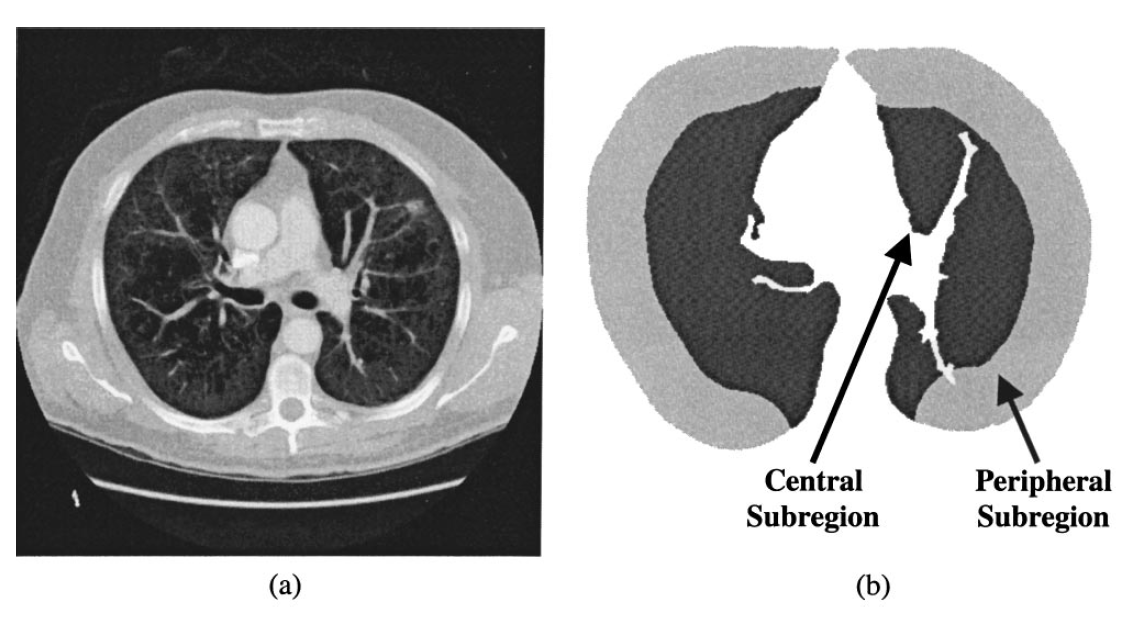
\includegraphics[scale=0.7]{gurcan_lungsegmentations.png}
\caption{This image is taken from Gurcan's paper ``Lung nodule detection on thoracic computed tomography images: Preliminary evaluation of a computer-aided diagnosis system''~\cite{gurcan2002lung} and shows the result of the segmentation process.}
\label{fig:segmentation}
\end{figure}


\subsection{Candidate Selection}
From the segmented lung region nodule candidates are selected. Nodule candidates should be distinct from blood vessels due to several morphological differences. 

- adaption of model parameters depending on a priori knowledge about the vessel density and the location of the slices

- candidates by intensity thresholding OR model fitting (geometrical or intensity models)

- sphericity might be a problem for juxtapleural nodules

- a multiple gray-level thresholding procedure, grouping pixels with similar intensity value and counting pixels in a connected neighborhood


\subsection{Classification}
The candidates have to be classified to separate cancerous nodules from non-malicious nodules. 

- LDA to distinguish the two classes

Link and describe in greater detail the approaches found in the classic filter selection pipelines.

Algorithm in this step would allow everyone of those to be



Firmino et.al~\cite{firmino2014computer} provide a very rich comparison of different CAD methods and their performance, which can be seen in Figure~\ref{fig:firmino_comp}

\begin{figure}[ht]
\centering
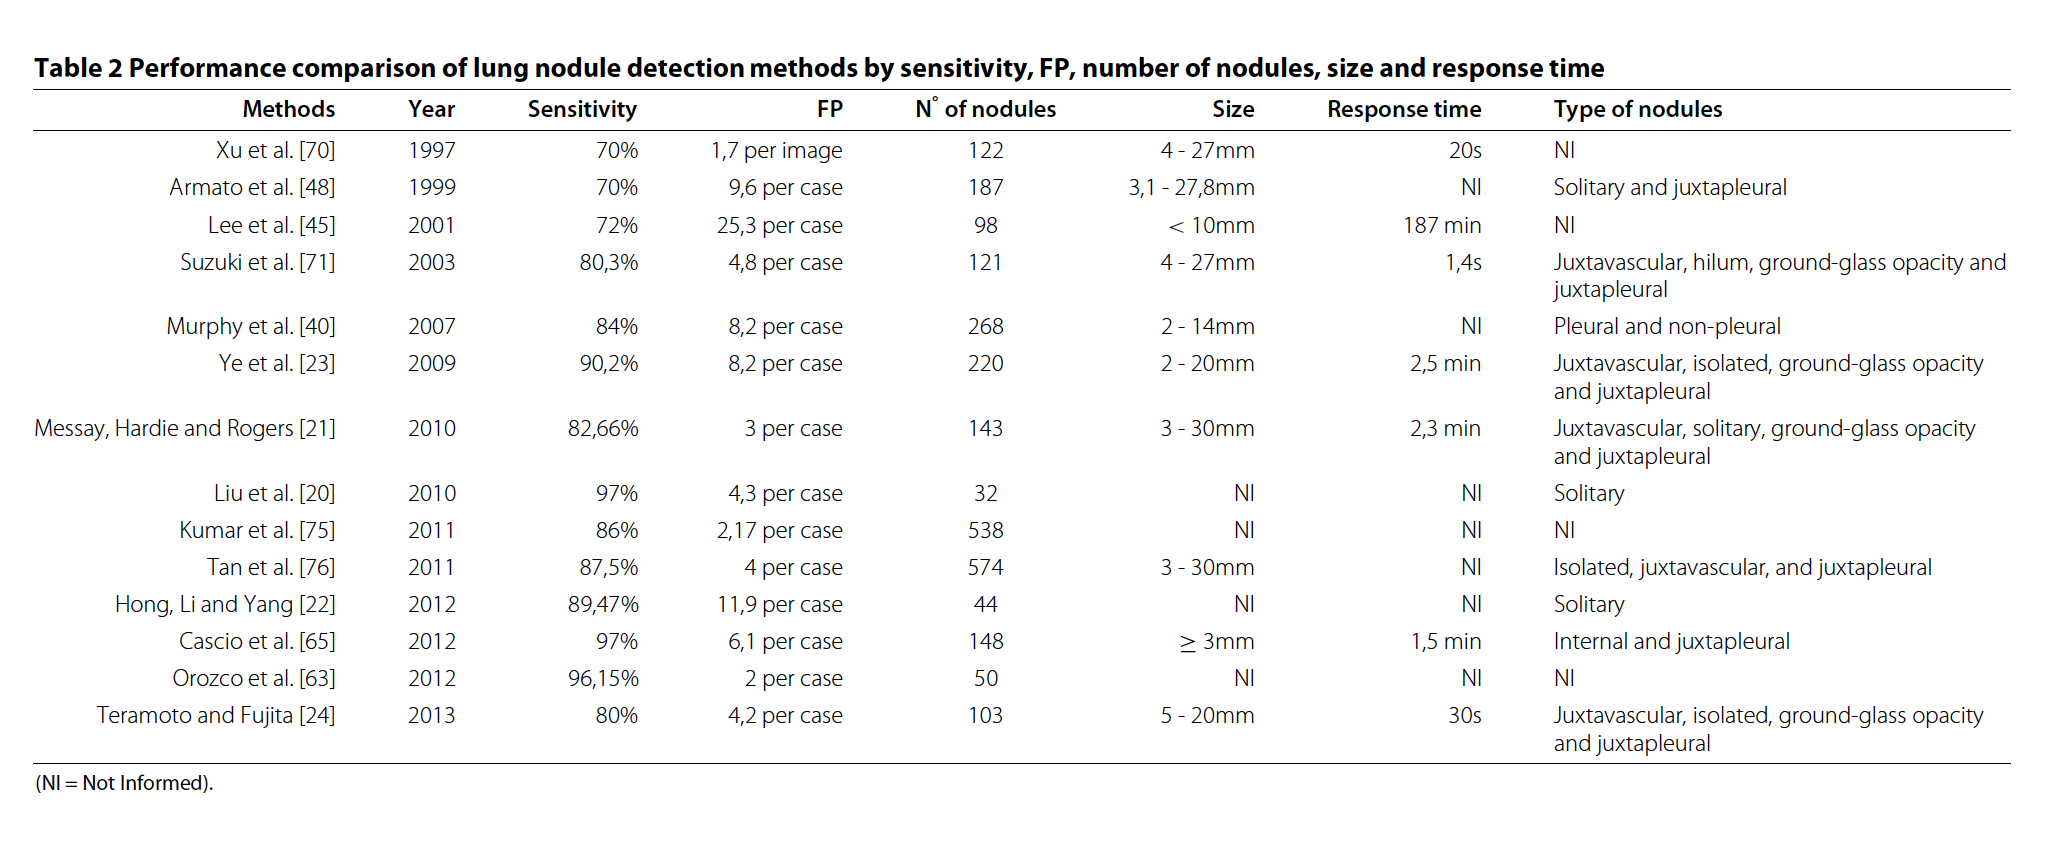
\includegraphics[width=\textwidth]{firmino_comparison.png}
\caption{This table is taken from Firmino et.al's paper ``Computer-aided detection system for lung cancer in computed tomography scans: Review and future prospects''~\cite{firmino2014computer} and shows the performance of different algorithms.}
\label{fig:firmino_comp}
\end{figure}

\section{Deep Learning Approaches}
Papers that deal with the neural network approach are explained here.

Mixture of approaches, taking the candidate selection and making the classification with statistical methods like neural networks (for this sake also LDA etc.)

\section{This Thesis}
Where can this thesis be positioned in the field of Lung CT analysis and nodule detection? Several  


Question: can lung nodule detection be done by neural networks? Can it be done by 3d convolutional neural networks? Can any further insight be gained from it?

Network only approach.

3D kernels for network. 

Nodule detection in the sense of yes/no not classification of other features like malignancy.


\end{document}
